\section{Onde d'urto}

Generalmente le onde d'urto utilizzate in trattamenti terapeutici sono
\textbf{onde ultrasonore} ad alta energia e alta pressione, che
raggiungono dei livelli molto alti di pressione, fino a 100 MPa
(megapascal), che equivalgono a 1000 bar. La loro velocità è superiore a
quella del suono.

\begin{figure}[!ht]
\centering
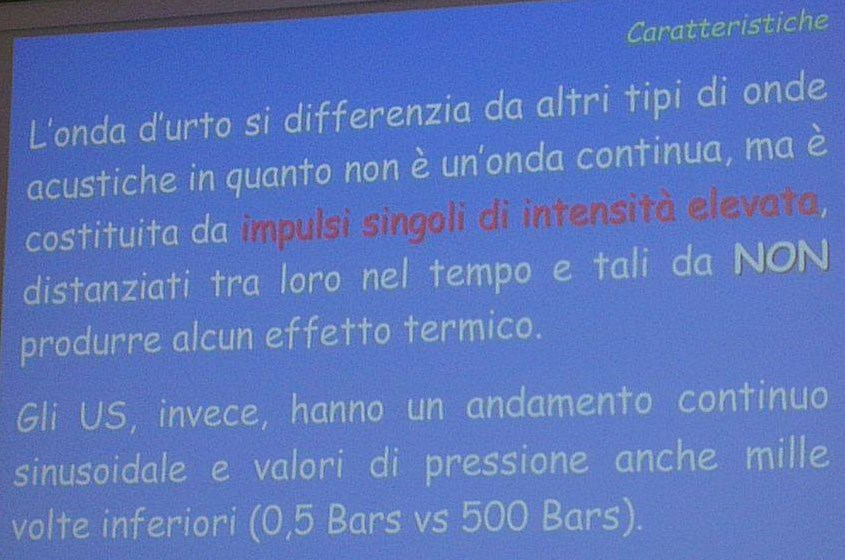
\includegraphics[width=0.4\textwidth]{025/image1.jpeg}
\end{figure}

Caratteristica fondamentale è l'\textbf{intensità} di questi impulsi,
che è elevata. Gli impulsi sono distanziati nel tempo, infatti nei
protocolli si utilizza un certo numero di ``colpi'': il \emph{colpo}
corrisponde a un impulso e tra un impulso e l'altro c'è una
\emph{pausa}.

Questi impulsi non producono effetto termico, anche se in realtà questa
affermazione è un po' discutibile: se io ho un effetto di compressione
su un tessuto, potrei in qualche modo avere un effetto termico a seconda
dell'intensità dell'impulso che utilizzo. Nello specifico, per non avere
un effetto termico, l'impulso deve essere velocissimo: se l'impulso ha
una velocità più bassa, si può avere un effetto termico. Per questa
ragione è stato concepito questo tipo di applicazione, per ridurre i
tipici effetti delle onde ultrasonore (come l'effetto termico) e
aumentare invece l'\textbf{effetto meccanico}.

C'è una notevole differenza tra la pressione esercitata da un'onda
ultrasonora senza scopo terapeutico e un'onda d'urto: 0,5 bar la prima e
500 bar la seconda.

L'andamento della pressione, che aumenta rapidamente, raggiunge il picco
e poi diminuisce in maniera ancora abbastanza rapida, fino ad arrivare a
valori negativi; poi si stabilizza.

Il decremento raggiunge -90 bar, mentre il picco raggiunge anche i 500
bar (in realtà potrebbe anche raggiungere i 1000 bar di picco, ma le
pressioni impiegate nel trattamento sono attorno ai 500).

Quindi le \textbf{caratteristiche} sono:

\begin{itemize}
\item
  elevata pressione di picco,
\item
  ciclo di durata brevissimo (inferiore a 10 $\mu$ s),
\item
  rapida salita (10 ns),
\item
  frequenza variabile da 16 Hz a 20 Mhz (da 16 hertz a 20 megahertz),
\end{itemize}

\begin{figure}[!ht]
\centering
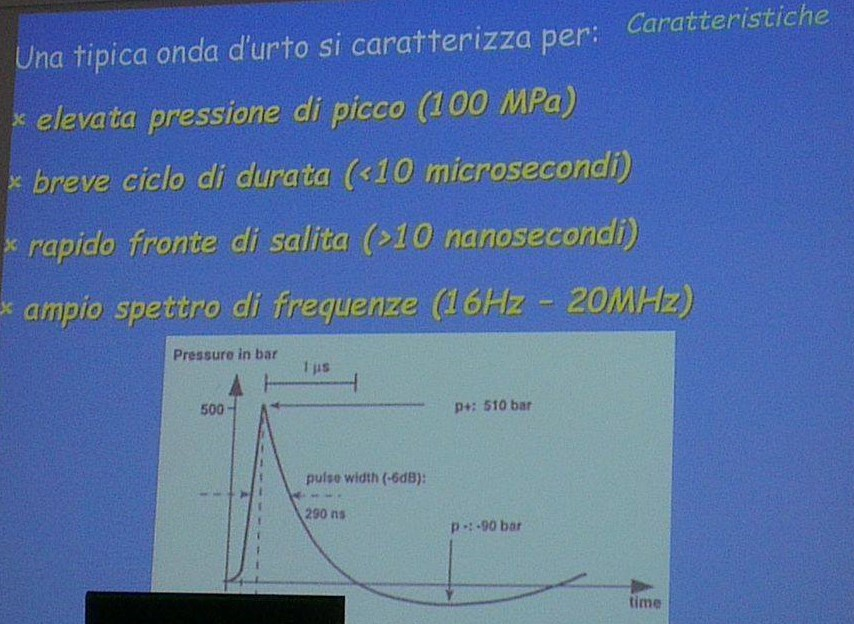
\includegraphics[width=0.4\textwidth]{025/image2.jpeg}
\end{figure}

La capacità di penetrare il tessuto dipende dalla caratteristica del
tessuto, dall'\textbf{impedenza tissutale} (definita impedenza acustica
a seconda del tipo di mezzo che si sta attraversando), che condiziona la
capacità di propagazione e l'intensità dell'onda.

L'importante è capire che l'onda d'urto deve attraversare dei tessuti e
a seconda del tipo di tessuto e anche della zona troverà maggiore o
minore resistenza: si pensi ad una coscia confrontandola con un bicipite
brachiale; la consistenza muscolare è diversa e quindi è diversa anche
la resistenza opposta dal tessuto. Ecco perché in alcune condizioni,
magari con trattamenti tipo ultrasuono, bisogna usare delle potenze più
alte.

Quindi i \textbf{parametri fondamentali} per stabilire qual è l'effetto
dell'onda d'urto sono:

\begin{itemize}
\item
  Pressione (in MPa),
\item
  Densità del flusso di energia (in mJ/mm\textsuperscript{2})
\item
  Energia totale (in mJ)
\end{itemize}

Una caratteristica dell'apparecchio a onde d'urto è quello di poter
concentrare il raggio in un punto ben preciso: questo punto è il
\textbf{focus} (o centro focale). Quindi l'onda d'urto si può puntare e
di fatto gli apparecchi utilizzati per i trattamenti sono spesso
supportati da \emph{controlli ecografici di puntamento}, per andare a
identificare perfettamente la zona e poterla colpire in maniera decisa.

\subsection{Generatori}

\begin{figure}[!ht]
\centering
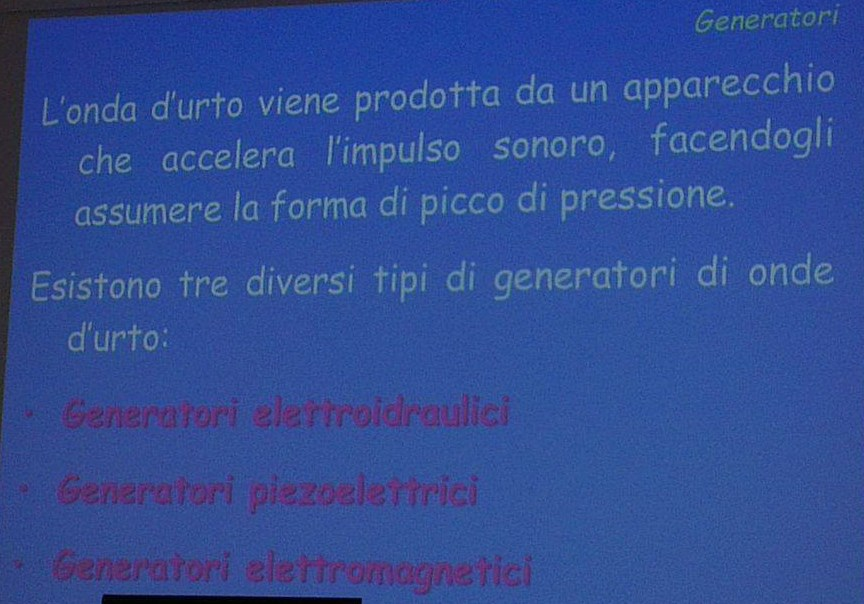
\includegraphics[width=0.4\textwidth]{025/image3.jpeg}
\end{figure}

È
importante sapere che esistono diverse forme di onde d'urto, diversi
apparecchi in circolazione:

\begin{itemize}
\item
  Elettroidraulici,
\item
  Piezoelettrici,
\item
  Elettromagnetici.
\end{itemize}

\begin{figure}[!ht]
\centering
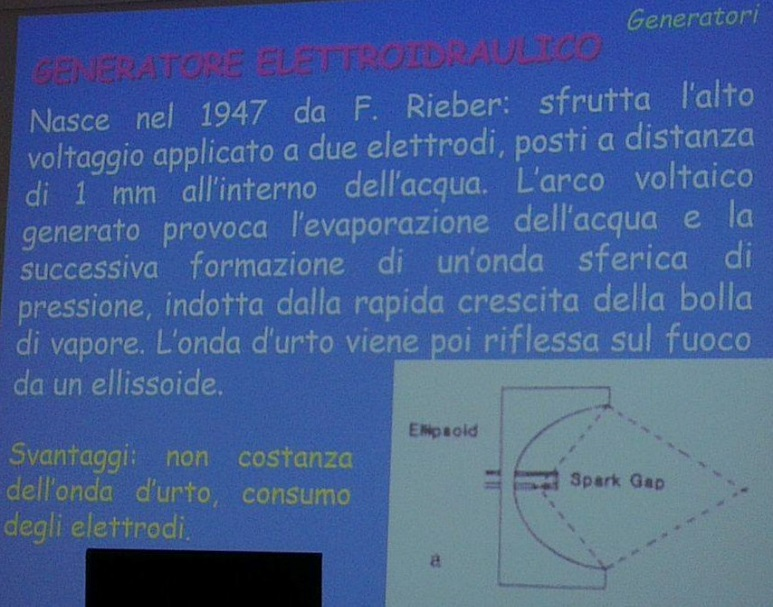
\includegraphics[width=0.4\textwidth]{025/image4.jpeg}
\end{figure}

\begin{itemize}
\item[1.]
  Se in casa si ha un compressore, magari lo si potrebbe utilizzare per
  creare un'onda d'urto per così dire ``artigianale'': accendendo e
  spegnendo si crea una potenza che si può definire tramite la
  regolazione del flusso (modificando l'ugello sulla punta del
  compressore) o tramite la taratura del compressore.

Gli apparecchi \textbf{elettroidraulici} sono di questo tipo e
utilizzati in questo modo. Lo svantaggio è che questo tipo di
apparecchio non mantiene il tipo di onda d'urto e quindi ha degli
\emph{sbalzi}, perciò possono esserci onde più o meno diverse; inoltre
hanno un \emph{elevato consumo degli elettrodi}. Si tratta infatti di
onda d'urto focale.

\begin{figure}[!ht]
\centering
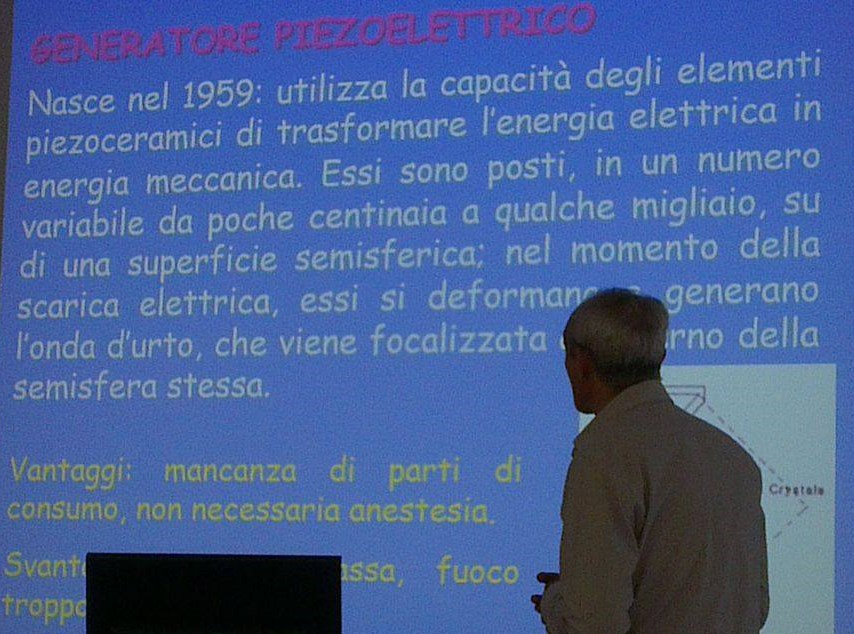
\includegraphics[width=0.4\textwidth]{025/image5.jpeg}
\end{figure}

\item
  Quello \textbf{piezoelettrico} ha una componente ceramica (che ha un
  effetto piezoelettrico). Un vantaggio è che questo tipo di generatore
  non crea una pressione sulla zona trattata tale da determinare una
  sintomatologia dolorosa: non è quindi necessario supportare questo
  tipo di trattamento con una contemporanea terapia farmacologica per il
  dolore (come invece occorre fare negli altri due casi).

Gli svantaggi sono invece la \emph{potenza bassa} e il \emph{fuoco
piccolo}.

\item[3.]
  Il generatore \textbf{elettromagnetico} ha un angolo di entrata molto
  limitato e quindi, al contrario del precedente, ha una
  \emph{dimensione del fuoco molto ampia}: questo, però, comporta anche
  effetti collaterali, perché ampliando la zona del fuoco ci possono
  essere lesioni nelle aree circostanti (si raggiungono picchi pressori
  molto elevati con problematiche locali).
\end{itemize}

Il generatore elettromagnetico ha la possibilità di agire in profondità.

\begin{figure}[!ht]
\centering
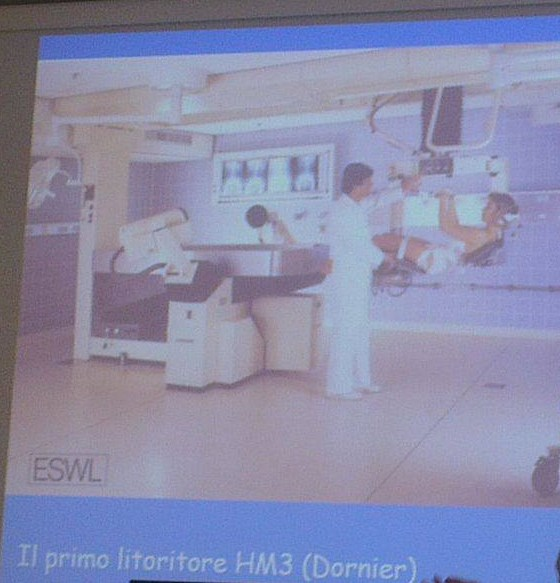
\includegraphics[width=0.4\textwidth]{025/image6.jpeg}
\end{figure}

L'apparecchio
che utilizzavano prima in urologia per trattare la calcolosi renale era
un apparecchio molto potente (un generatore elettromagnetico di prima
generazione);

adesso usano invece un apparecchio diverso che ha un fuoco meno potente,
ha la possibilità di identificare la zona da bombardare e ha un
cuscinetto di acqua su cui il paziente si posiziona per assorbire
l'onda.

Questo però ha portato ad avere un apparecchio che non ha più la potenza
di quello di una volta (più bassa di almeno un 30\%): ha un sistema
generatore abbastanza diverso che per alcuni aspetti non è più adeguato
perché necessita di un maggior numero di colpi e un trattamento
prolungato per più sedute. Inoltre non ha neanche un puntamento
ecografico adeguato.

È successo che non si sia riusciti a bombardare un calcolo sviluppatosi
in un paziente dello stesso tipo e con le stesse consistenza e
localizzazione di un calcolo precedentemente trattato con il vecchio
apparecchio.

Il \textbf{sistema di puntamento} è importante:

\begin{itemize}
\item
  con un \textbf{puntamento ecografico} è sicuramente identificabile il
  punto da trattare.
\item
  i \textbf{puntamenti radiografici} ormai non si usano più, perché sono
  certamente più utili quelli ecografici
\item
  oppure ci sono gli apparecchi idropneumatici che non hanno alcun tipo
  di puntamento:

\begin{itemize}
\item
  si chiede al paziente dove ha dolore e ci si basa su \emph{esami
  radiologici} effettuati in precedenza per individuare la zona da
  trattare;
\item
  altrimenti ci si può basare semplicemente sulla conoscenza della zona.

Per esempio, se c'è un tendine d'Achille particolarmente ispessito o
degenerato si fanno delle onde d'urto nella zona corrispondente, per
rivascolarizzare l'area (dal momento che queste onde stimolano la
neoangiogenesi): il tendine dovrebbe trarre beneficio dal maggior
afflusso di sangue perché verrebbe a ridursi la condizione di
degenerazione (a volte prima si ha ispessimento, poi subentra la
degenerazione, con riduzione delle resistenze e quindi rottura).
\end{itemize}
\end{itemize}
Le onde d'urto sono state anche utilizzate nei ritardi di
\emph{consolidazione delle fratture} ma con scarso beneficio, mentre
sono sicuramente più efficaci nelle forme in cui c'è una
\emph{pseudoartrosi} (andando a rompere le aderenze).

\begin{figure}[!ht]
\centering
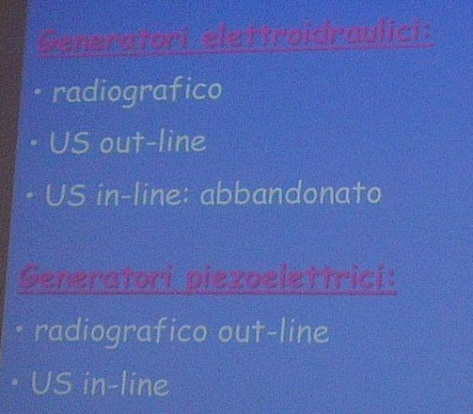
\includegraphics[width=0.4\textwidth]{025/image7.jpeg}
\end{figure}

Nei generatori elettroidraulici ci può essere un puntamento radiografico
o ecografico, così come nei generatori piezoelettrici. Che sia
all'interno o all'esterno ha poca importanza.

\begin{figure}[!ht]
\centering
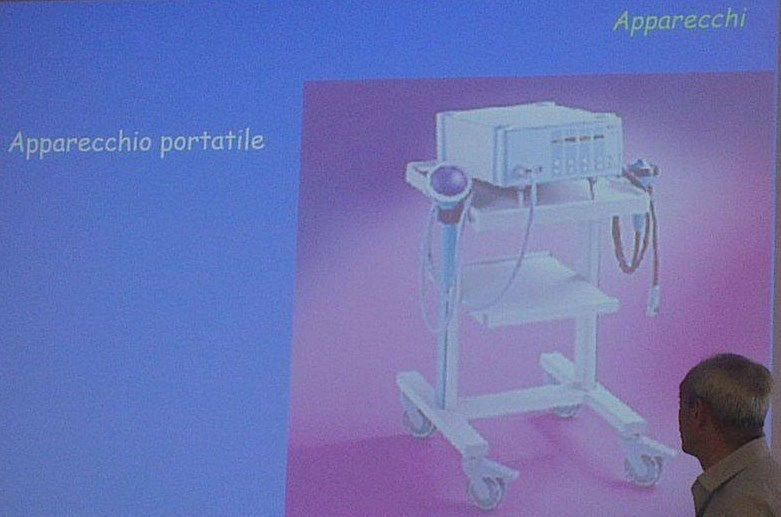
\includegraphics[width=0.4\textwidth]{025/image8.jpeg}
\end{figure}

Per
quanto riguarda gli apparecchi, ci sono sistemi abbastanza ingombranti e
sistemi addirittura portatili. Quelli idropneumatici sono portatili
perché non hanno nessuno controllo ecografico e sono quindi abbastanza
semplici da utilizzare.

\begin{figure}[!ht]
\centering
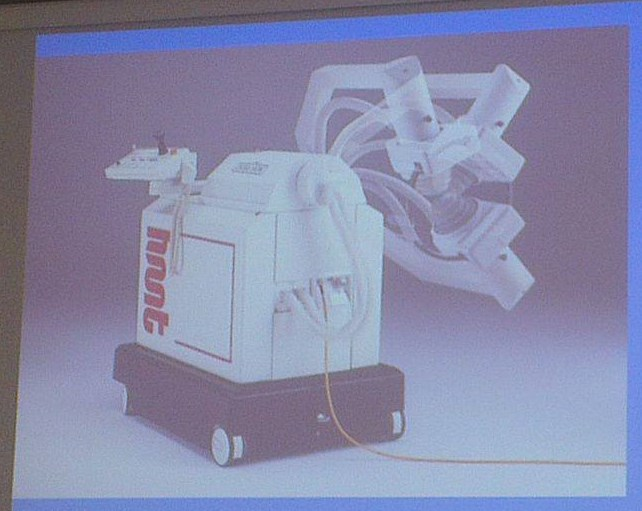
\includegraphics[width=0.4\textwidth]{025/image9.jpeg}
\end{figure}

Questo è un apparecchio (OssaTron) utilizzato in ambito ortopedico che
permette un'applicazione mobile (rotazione di 350\textsuperscript{o}).

Ci sono apparecchi più complianti di ultima generazione che però sono
meno efficaci perché non hanno il puntatore e il generatore è
idropneumatico.

\begin{figure}[!ht]
\centering
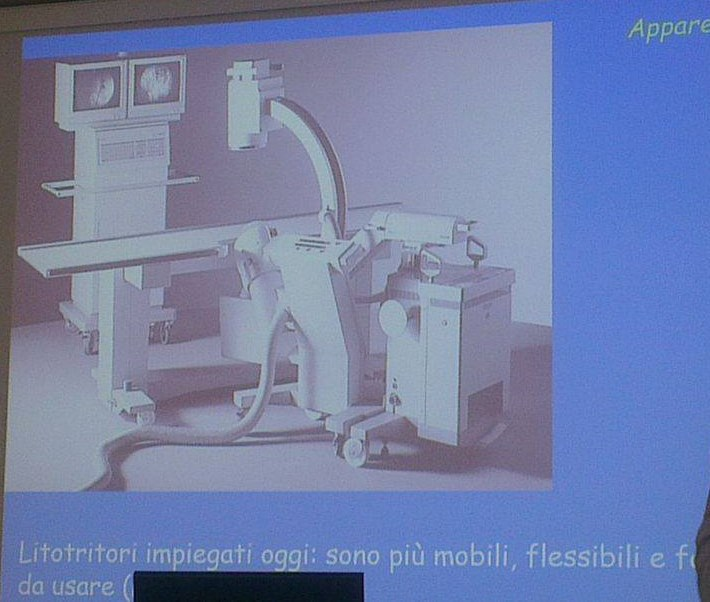
\includegraphics[width=0.4\textwidth]{025/image10.jpeg}
\end{figure}

Ovviamente l'effetto è sempre quello tipico dell'ultrasuono:
\emph{riflessione}, \emph{trasmissione}, \emph{assorbimento}. Si ha
quindi questa sollecitazione importante creando delle zone di trazione,
compressione e rarefazione.

L'effetto meccanico è tipico dell'onda d'urto perché c'è un'assenza
dell'effetto termico:

l'\textbf{effetto meccanico} può essere:

\begin{itemize}
\item
  \textbf{diretto} (l'onda d'urto agisce con un sistema di compressione
  e retrazione all'interfaccia dei tessuti, a seconda della densità e
  dell'impedenza acustica del tessuto)
\item
  \textbf{indiretto}, tipico dell'ultrasuono, cioè l'effetto meccanico
  per eccellenza che è la \emph{cavitazione}, ossia la formazione di
  bolle di gas che poi tendono a rompersi, determinando una
  microemorragia, una petecchia emorragica che stimola la rigenerazione
  tissutale (neoangiogenesi).

Si creano microlesioni, in base al numero degli impulsi e all'energia
erogata e alla resistenza offerta dal tessuto (concentrazione di acqua
nel tessuto). {[}L'apparecchio che c'è ora in urologia, che ha una bolla
d'acqua posizionata sotto al paziente, tende ad adsorbire ancora di più
l'onda e quindi non permette all'onda stessa di esprimere il potenziale
che ha (cioè la potenza adeguata).{]}
\end{itemize}

\begin{figure}[!ht]
\centering
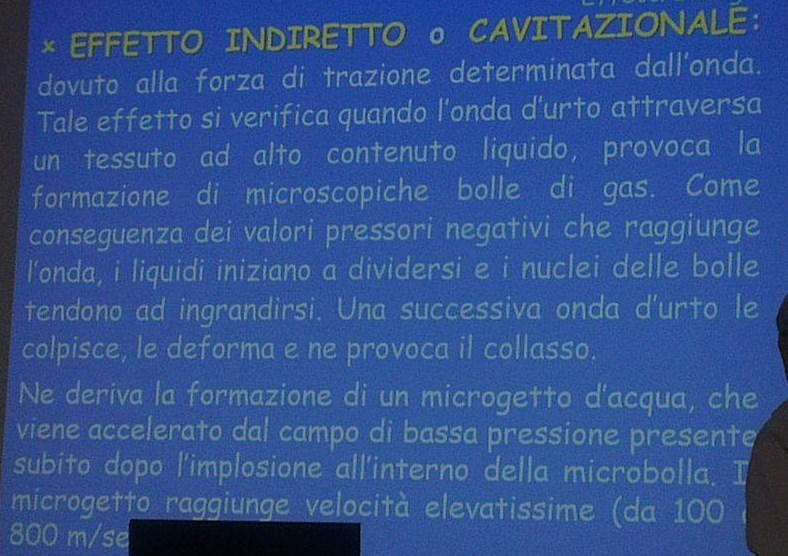
\includegraphics[width=0.4\textwidth]{025/image11.jpeg}
\end{figure}

\begin{figure}[!ht]
\centering
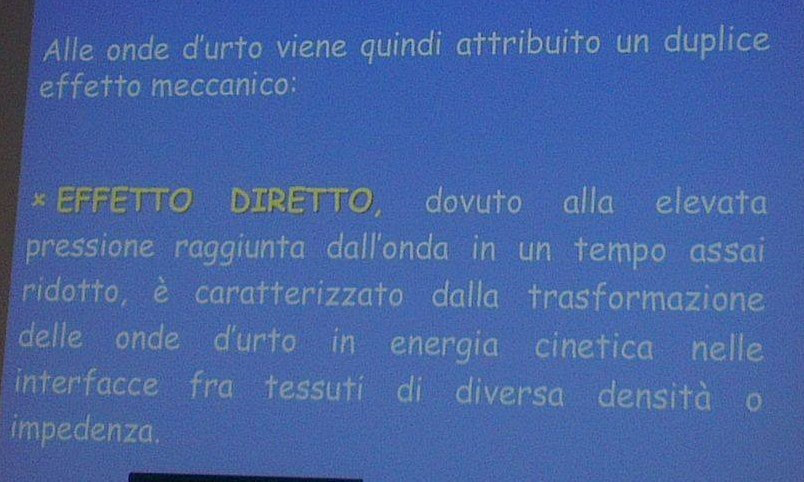
\includegraphics[width=0.4\textwidth]{025/image12.jpeg}
\end{figure}

\begin{figure}[!ht]
\centering
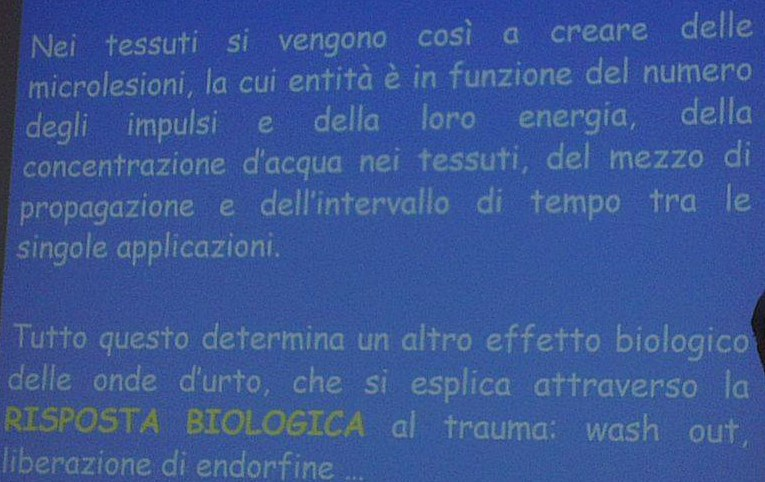
\includegraphics[width=0.4\textwidth]{025/image13.jpeg}
\end{figure}

\begin{figure}[!ht]
\centering
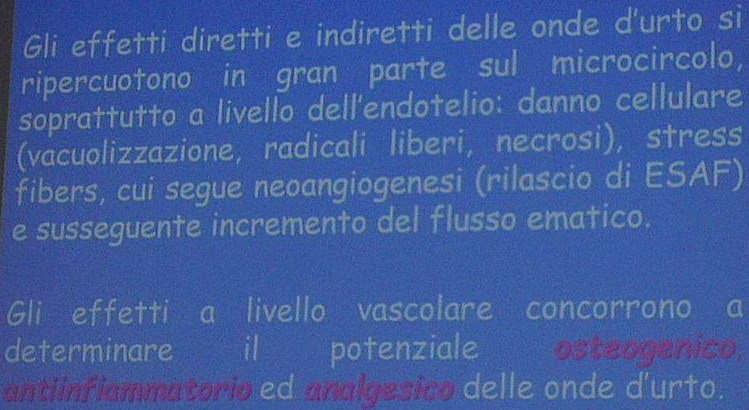
\includegraphics[width=0.4\textwidth]{025/image14.jpeg}
\end{figure}

La risposta biologica al trattamento con l'onda d'urto è il cosiddetto
\textbf{wash-out}, cioè la pulizia della zone, quindi la rimozione di
tutte le sostanze tipiche del processo infiammatorio (con la liberazione
di endorfine).

\begin{figure}[!ht]
\centering
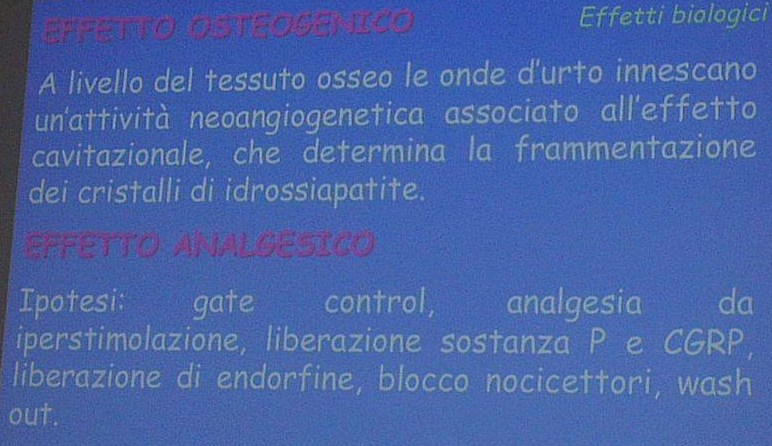
\includegraphics[width=0.4\textwidth]{025/image15.jpeg}
\end{figure}

Ci
sono poi effetti importanti a livello vascolare, con \textbf{azione:}

\begin{itemize}
\item
  \textbf{antinfiammatoria}
\item
  \textbf{analgesica}: si ritiene dovuta all'apertura dei canali e
  quindi attraverso un \emph{controllo centrale} per cui vengono
  liberate localmente delle sostanze importanti e s'impedisce la
  trasmissione dell'impulso doloroso attraverso la via dolorifica che
  passa per le corna posteriori del midollo spinale (stesso meccanismo
  dell'elettroterapia antalgica; qualsiasi tipo di trattamento locale
  ha, infatti, un effetto di retroazione delle endorfine).
\item
  \textbf{osteogenetica} (apposizione di callo osseo per stimolazione
  degli osteoblasti): \emph{l'attività è neoangiogenetica, associata
  all'effetto cavitazionale} con \emph{frammentazione dei cristalli di
  idrossiapatite} (è il complesso della riparazione tissutale, che può
  avvenire per sostituzione del tessuto o per formazione di nuove
  cellule). Di sicuro si forma il \emph{tessuto di granulazione}.
\end{itemize}

\begin{figure}[!ht]
\centering
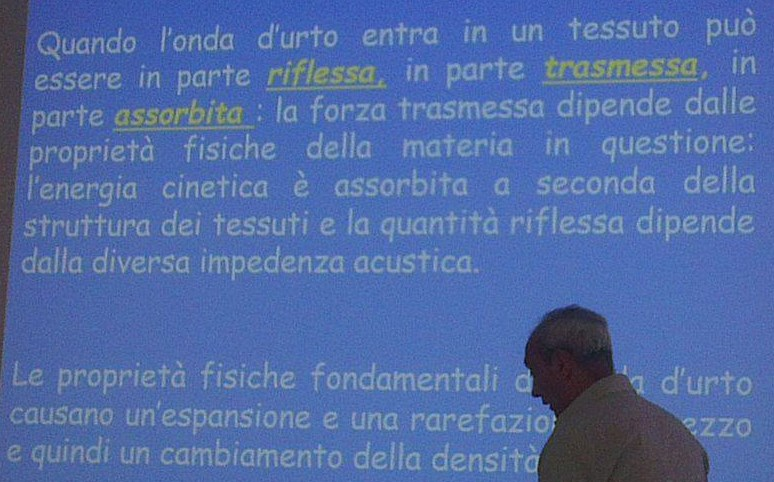
\includegraphics[width=0.4\textwidth]{025/image16.jpeg}
\end{figure}

\subsection{Indicazioni alle onde d'urto}

Possono essere utilizzate per la \textbf{frammentazione di
calcificazioni} (tendinopatie calcifiche). L'efficacia dipende dal tipo
e della composizione della calcificazione:

\begin{itemize}
\item
  più efficace sulle calcificazioni di \emph{carbonato}
\item
  per quelle di \emph{ossalato} si ha un livello di efficacia intermedio
\item
  è nulla per quelle di \emph{fosfato}.

Per questa ragione adesso si utilizza una nuova tecnica, che è quella
del doppio lavaggio: in questo modo le calcificazioni si lavano via (lo
fanno i radiologi, soprattutto nelle patologie di spalla più
resistenti).
\end{itemize}

\begin{figure}[!ht]
\centering
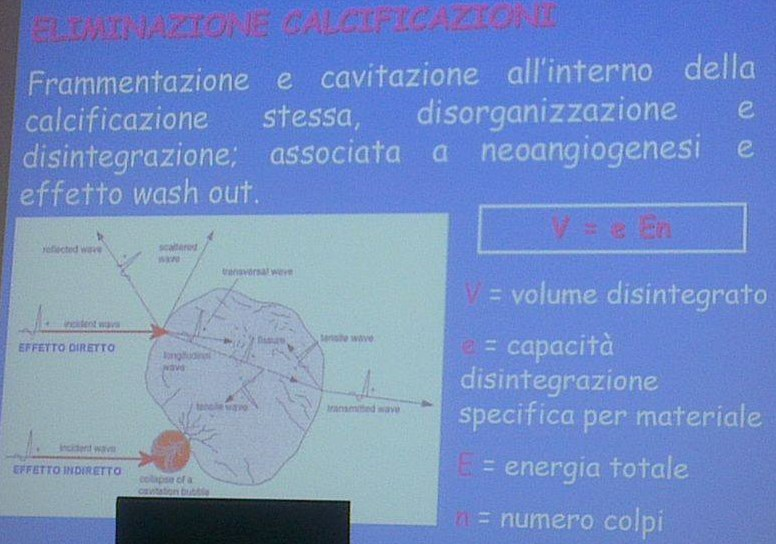
\includegraphics[width=0.4\textwidth]{025/image17.jpeg}
\end{figure}

L'effetto dipende dal \textbf{numero di colpi} e dalla \textbf{dose}
utilizzata, che è diversa a seconda della patologia che si sta
trattando:

\begin{itemize}
\item
  dosi elevate per i processi di pseudoartrosi e ritardi di
  consolidazione
\item
  dosi medie nelle tendinosi con calcificazione
\item
  dosi basse per le patologie tendinee.
\end{itemize}

\begin{figure}[!ht]
\centering
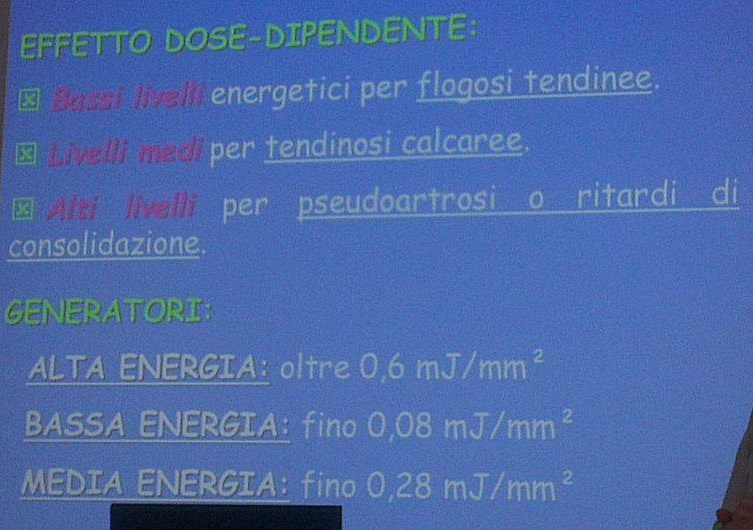
\includegraphics[width=0.4\textwidth]{025/image18.jpeg}
\end{figure}

Ultimamente medici di Napoli e Roma si sono interessati all'impiego di
onde d'urto per trattare muscoli spastici dell'arto superiore, ottenendo
grandi benefici, perché l'effetto meccanico è quasi sovrapponibile ad un
effetto vibratorio: se si modula questo effetto in maniera adeguata e si
fa in modo che la dose di applicazione sia di livello medio-basso, si
hanno risultati veramente interessanti.

L'energia è variabile e può essere considerata importante in base
all'applicazione che viene fatta.

Oltre ad applicazioni già conosciute in passato, ha avuto uno sviluppo
notevole in ambito ortopedico e nelle patologie dell'apparato
locomotore, tant'è vero che esiste una società italiana delle onde
d'urto con un'enorme produzione scientifica.

\subsubsection{Applicazioni}

Queste sono le patologie più importanti in cui è stato usato un
trattamento con le onde d'urto:

\begin{itemize}
\item
  Litotrissia extracorporea
\item
  Malattia di Peyronie
\item
  Litiasi biliare
\item
  Affezioni dell'apparato locomotore:
\item
  Pseudoartrosi e ritardo di consolidazione
\end{itemize}

\begin{figure}[!ht]
\centering
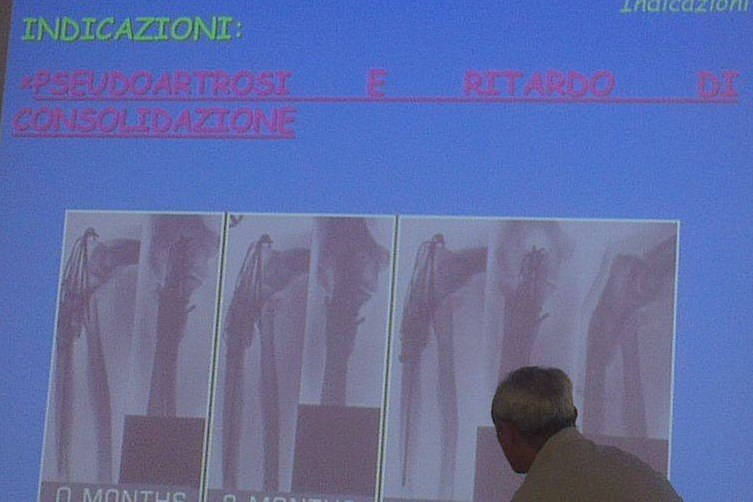
\includegraphics[width=0.4\textwidth]{025/image19.jpeg}
\end{figure}

\begin{figure}[!ht]
\centering
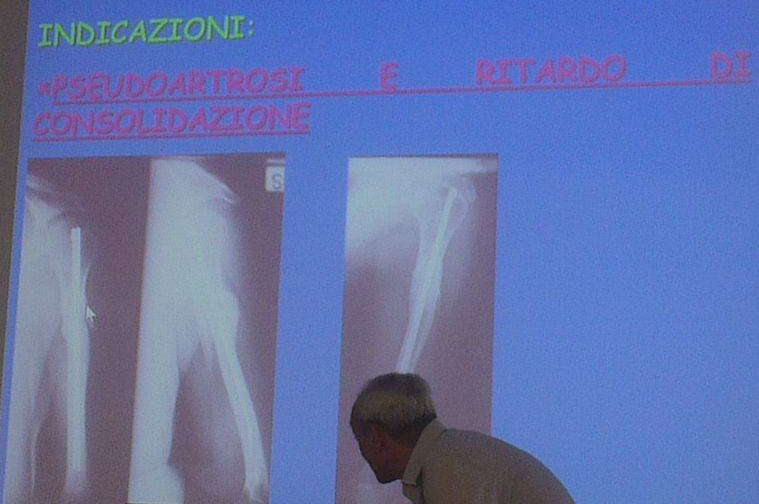
\includegraphics[width=0.4\textwidth]{025/image20.jpeg}
\end{figure}

Questo trattamento ha permesso la maggior apposizione di callo osseo con
rimodellamento.

\subsubsection{Altre applicazioni}

\begin{itemize}
\item
  tendinopatie calcifiche della spalla
\item
  epicondilite
\item
  epitrocleite
\item
  sperone calcaneare
\item
  fascite plantare
\item
  tendinopatia achillea
\item
  tendinopatia rotulea
\item
  pubalgia
\item
  \emph{necrosi asettica della testa femorale:} oltre a trattamenti
  quali l'iperbarica, anche la stimolazione con onde d'urto può essere
  d'aiuto; ovviamente bisogna stare attenti a non creare situazioni
  ancora peggiori.

Si riporta l'esempio di un ragazzo di 24 anni con necrosi della testa
omerale causata da chemioterapia: dopo un trattamento con le onde d'urto
e l'iperbarica ha avuto un enorme beneficio).

\item
  paraosteoartropatia.
\item
  Per le \textbf{lesioni muscolari} ci sono aspetti contraddittori:
  alcuni medici le consigliano, altri no, soprattutto nelle fasi
  iniziali.

In ogni caso il trattamento non va iniziato prima di 72 ore e se ci sono
rotture ed ematomi.

\item
  Invece nelle \textbf{contratture} e nelle \textbf{elongazioni}
  (stiramenti) senza rotture, si possono utilizzare senza problemi.

\begin{figure}[!ht]
\centering

\includegraphics[width=0.4\textwidth]{025/image21.jpeg}
\end{figure}

\item
  Sono impiegate anche nei casi di \textbf{osteocondrite dissecante} e
  \textbf{algodistrofie} (soprattutto perché l'onda d'urto ha un effetto
  importante sui nocicettori e in una forma come l'algodistrofia la
  modulazione del dolore è importante).
\end{itemize}

\subsection{Controindicazioni}

\begin{figure}[!ht]
\centering
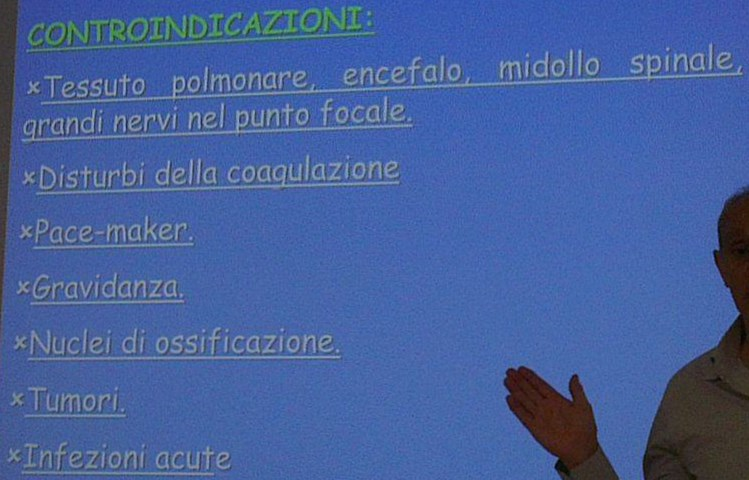
\includegraphics[width=0.4\textwidth]{025/image22.jpeg}
\end{figure}

Come in tutti i trattamenti terapeutici strumentali esistono delle
controindicazioni:

\begin{itemize}
\item
  innanzitutto, è bene che non si trovino \emph{tessuto polmonare,
  encefalo, midollo spinale e grandi nervi} nel punto focale.

Se si tratta, per esempio, la testa del perone in un paziente con
diagnosi di bendelletta ileotibiale, occorre fare molta attenzione
perché lì passa lo \textbf{SPE} (nervo sciatico popliteo esterno) e, se
colpito, il soggetto si può ritrovare con un piede cadente.

\item
  \emph{Pace-maker}, \emph{gravidanze} e \emph{tumori} sono tipiche
  controindicazioni delle terapie strumentali in generale.
\item
  \emph{Disturbi della coagulazione}: dal momento che l'onda d'urto crea
  una cavitazione (la bolla di gas si rompe), questo può peggiorare il
  discorso del sanguinamento.
\item
  In corso di \emph{infezioni acute}.
\item
  Sui \emph{nuclei di ossificazione} sarebbe controindicato ma alcuni le
  usano: nella fase avanzata, quando dovrebbe esserci il passaggio dalla
  forma fibrosa alla forma ossea, con dosaggi bassi potrebbe anche
  essere utile; altrimenti è più consigliata la termoterapia.
\end{itemize}

\subsection{Effetti collaterali}

\textbf{Aumento del} \textbf{dolore}: \emph{l'onda d'urto fa male.}

Il trattamento non è giornaliero, va fatto a distanza di tempo per un
numero di sedute non elevato, per un tempo adeguato. L'effetto
terapeutico si manifesta a distanza di tempo, perché nell'immediato c'è
l'effetto meccanico doloroso.

Altri effetti collaterali sono \textbf{petecchie e microematomi}.

\begin{figure}[!ht]
\centering
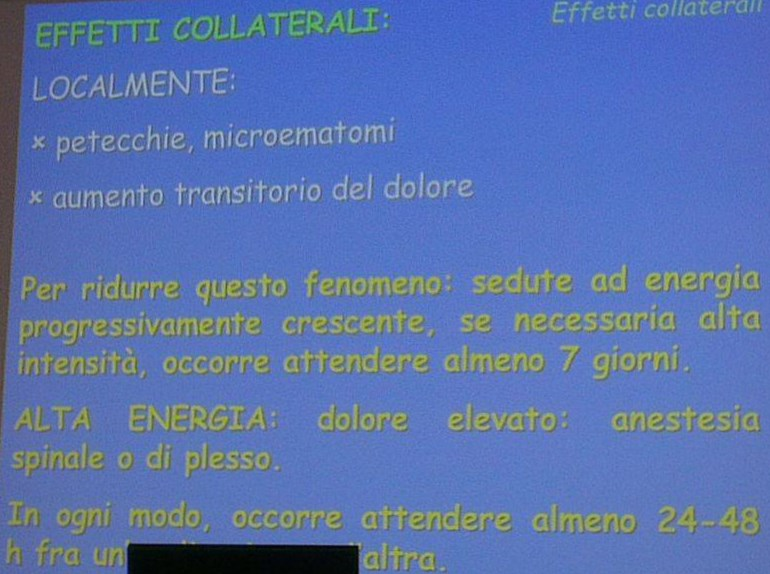
\includegraphics[width=0.4\textwidth]{025/image23.jpeg}
\end{figure}

\begin{figure}[!ht]
\centering
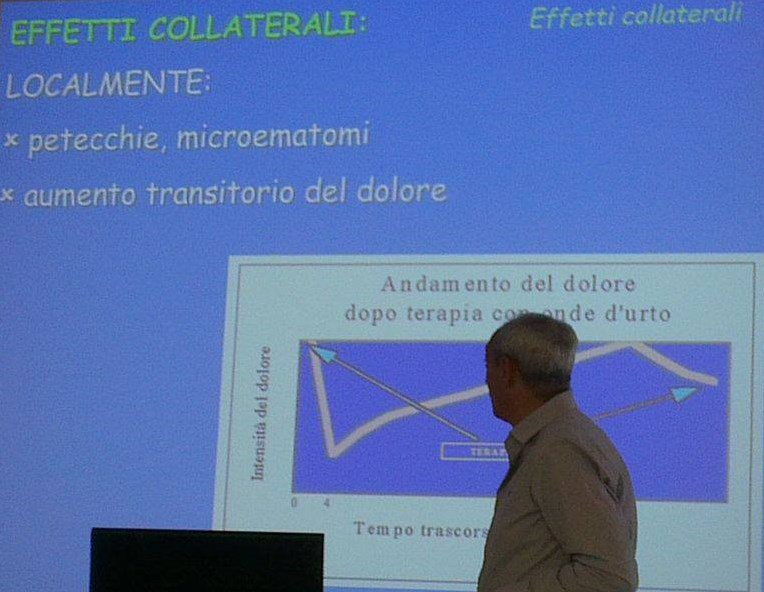
\includegraphics[width=0.4\textwidth]{025/image24.jpeg}
\end{figure}

Per ridurre gli effetti collaterali, si può procedere con sedute ad
energia progressivamente crescente, a 7 giorni di distanza tra un
trattamento e l'altro (mai meno di 48 ore tra un trattamento e l'altro),
in media tre trattamenti totali.

Se è necessario utilizzare alta energia, bisogna utilizzare sicuramente
un \textbf{trattamento farmacologico per il dolore} (in urologia usavano
il Fentanest).

Si può usare l'anestesia: locale, spinale e di plesso (questa, però,
diventa complessa).

È ovvio che per usare le onde d'urto bisogna avere un livello di
conoscenza elevato del loro utilizzo: la legge prevede che siano
utilizzate da medici, così come è previsto per il laser ad alta potenza.

Solo le forme, per così dire, meccaniche (senza puntamento), vengono
utilizzate anche da personale non medico, per cui si trovano in diversi
studi di riabilitazione.

\textbf{Esempio di protocollo} (peraltro abbastanza intenso) per
calcificazione di spalla: 4 sedute, 2500 colpi, 120 colpi al minuto.

È un po' come i trattamenti che agiscono sulla fascia (come i
trattamenti di massaggio connettivale), che sono molto dolorosi ma poi
danno un effetto terapeutico importante (che non è immediato) o altre
tecniche come, per esempio, il rolfing, che prevedono un aumento della
vascolarizzazione locale.

\subsection{Confronto con altri trattamenti}

Anche per la \emph{magnetoterapia} si era parlato degli \textbf{effetti
neoangiogenetico} e \textbf{osteogenetico}.

Innanzitutto val la pena riportare l'esempio dei tendini: il tendine in
maniera autonoma rigenera, facendo esattamente tutto quello che produce
l'onda d'urto in maniera naturale.

Ad oggi si utilizzano le onde d'urto perché non si conoscono ancora
perfettamente i meccanismi alla base della riparazione naturale dei
tendini (non abbiamo ancora studi genetici a questo scopo): se si
sapessero, basterebbe modulare l'azione del tendine, mettendolo
semplicemente nelle condizioni ideali per esplicare questo meccanismo in
maniera automatica.

Se c'è un ritardo di consolidazione è preferibile utilizzare la
magnetoterapia perché ci sono molti più risultati (sicuramente con i
magneti naturali, rispetto alla magnetoterapia classica che c'è adesso).

Per quanto riguarda le onde d'urto nei \textbf{ritardi di
consolidazione}, forse negli ultimi cinque anni qualcosa è migliorato,
perché ci sono degli apparecchi nuovi prodotti da aziende, tra le quali
l'Igea, che è stata l'unica in Italia che è riuscita ad emergere nella
rivisitazione internazionale dei trattamenti dei campi biomagnetici in
terapia clinica.

In linea generale, però, onde d'urto nei ritardi di consolidazione non
trovano applicazione.

Anche per le \textbf{calcificazioni} ci sono altre tecniche:

\begin{itemize}
\item
  una può essere il \emph{doppio lavaggio} che si fa in controllo
  radioscopico
\item
  poi c'è anche la possibilità di utilizzare farmaci che agiscono
  localmente, come per esempio l'\emph{EDTA sale bisodico} (il sale
  monosodico è quello che si usa invece nelle provette per evitare la
  coagulazione), che è un chelante del calcio: se iniettato localmente
  in maniera adeguata con tecniche di mesoterapia con una diluizione
  particolare, brucia ma funziona perché le calcificazioni scompaiono.

Il problema di fondo è però se la calcificazione sia dolorosa o meno:
molti ritengono che non lo sia e che il dolore sia legato ad altri
aspetti (derivi dalla modulazione di altre situazioni).
\end{itemize}

In buona sostanza, se devo avere un effetto biostimolante preferisco la
\textbf{magnetoterapia} perché è più semplice da utilizzare: il paziente
se la può fare a casa, è più compliante.

Anche il costo è più basso rispetto alle onde d'urto, anche se occorre
un maggior numero di sedute.

Il sistema sanitario nazionale non convenziona né le onde d'urto né la
magnetoterapia (quest'ultima potrebbe essere fatta in convenzione in
casi particolari con un progetto riabilitativo personalizzato entro sei
mesi da un intervento chirurgico, così come l'elettrostimolazione).
